%%%%%%%%%%%%%%%%%%%% author.tex %%%%%%%%%%%%%%%%%%%%%%%%%%%%%%%%%%%
%
% sample root file for your "contribution" to a contributed volume
%
% Use this file as a template for your own input.
%
%%%%%%%%%%%%%%%% Springer %%%%%%%%%%%%%%%%%%%%%%%%%%%%%%%%%%


% RECOMMENDED %%%%%%%%%%%%%%%%%%%%%%%%%%%%%%%%%%%%%%%%%%%%%%%%%%%
\documentclass[graybox]{svmult}

% choose options for [] as required from the list
% in the Reference Guide

\usepackage{type1cm}        % activate if the above 3 fonts are
                            % not available on your system
%
\usepackage{makeidx}         % allows index generation
\usepackage{graphicx}        % standard LaTeX graphics tool
                             % when including figure files
\usepackage{multicol}        % used for the two-column index
\usepackage[bottom]{footmisc}% places footnotes at page bottom


\usepackage{newtxtext}       % 
\usepackage[varvw]{newtxmath}       % selects Times Roman as basic font
\usepackage{needspace}
\usepackage{titlesec}
\usepackage{float}

\graphicspath{{figures/}}



% see the list of further useful packages
% in the Reference Guide

\makeindex             % used for the subject index
                       % please use the style svind.ist with
                       % your makeindex program

%%%%%%%%%%%%%%%%%%%%%%%%%%%%%%%%%%%%%%%%%%%%%%%%%%%%%%%%%%%%%%%%%%%%%%%%%%%%%%%%%%%%%%%%%

\begin{document}

\title*{Smart home control app using Home Assistant}
% Use \titlerunning{Short Title} for an abbreviated version of
% your contribution title if the original one is too long
\author{José Guedes, Nelson Fernandes, Pedro Filipe Oliveira and Paulo Matos}
% Use \authorrunning{Short Title} for an abbreviated version of
% your contribution title if the original one is too long
\institute{José Guedes \at Instituto Politécnico de Bragança, Portugal, \email{a56576@alunos.ipb.pt}
\and Nelson Fernandes \at Instituto Politécnico de Bragança, Portugal, \email{a51796@alunos.ipb.pt}
\and
Pedro Filipe Oliveira \at CeDRI, SusTEC, Instituto Politécnico de Bragança, 5300-253 Bragança, Portugal \email{poliveira@ipb.pt}
\and Paulo Matos \at CeDRI, SusTEC, Instituto Politécnico de Bragança, 5300-253 Bragança, Portugal \email{pmatos@ipb.pt}}

%\and
%Miguel Mira da Silva \at Instituto Superior Técnico, University of Lisbon, Lisbon, Portugal, \email{mms@tecnico.ulisboa.pt}}
%
% Use the package "url.sty" to avoid
% problems with special characters
% used in your e-mail or web address
%
\maketitle

%Each chapter should be preceded by an abstract (no more than 200 words) that summarizes the content. The abstract will appear \textit{online} at \url{www.SpringerLink.com} and be available with unrestricted access. This allows unregistered users to read the abstract as a teaser for the complete chapter.
%Please use the 'starred' version of the \texttt{abstract} command for typesetting the text of the online abstracts (cf. source file of this chapter template \texttt{abstract}) and include them with the source files of your manuscript. Use the plain \texttt{abstract} command if the abstract is also to appear in the printed version of the book.}

\abstract{Technology areas continue to generate high interest and financial investment, with home automation being one of the fields that has grown the most in recent years. This growth is justified by the increase in IoT devices, and people's interest in modernizing their homes, seeking greater comfort and convenience for their residents.
Despite this rapid evolution, we still find several obstacles in the application of home automation in smart homes, the lack of compatibility between brands, the dependence on cloud services, and a high initial cost are some of the barriers that hinder its widespread adoption.
With this problem in mind, a simple and practical system was planned that would allow, in a centralized way, to control various aspects of a residential home. For this project, the open-source platform Home Assistant was chosen to monitor energy consumption, control thermostats and manage video surveillance cameras of a residential home.
All the development of this solution is based on a centralized system, through the Home Assistant interface. Communication between smart devices is carried out exclusively through Wi-Fi connectivity, ensuring a simple and wireless configuration.
This project, based on Home Assistant, provides users with greater comfort, security and management of their home's energy resources, ensuring a more practical and sustainable experience. One of the major strengths of Home Assistant is the fact that it runs locally on the network, ensuring total data privacy.\\
Key words: automation, home assistant, open source, privacy.
}



\section{Introduction}\label{sec:intro}

It is undeniable that, in recent years, the smart device market has grown at an accelerated pace. The increase in home automation solutions, driven by the popularization of smart homes and the interest in controlling households, is among the main reasons. These smart devices are increasingly becoming part of our daily lives, improving the way we interact with the home, providing greater comfort to users, as well as management of energy consumption and home security. The instability in energy prices and a greater environmental concern have led consumers to seek IoT solutions that allow a more rational use of resources.
Despite this growth in IoT devices and the high level of interest from people, many users still face difficulties in integrating and configuring them with the chosen platform. There is often a lack of compatibility between the chosen platform and the IoT devices. To solve these problems, Home Assistant emerged as an open-source solution that has a vast list of compatible devices and a large community that develops and maintains the integrations. One of the strong points of this platform is the fact that it does not depend on external services, which ensures total privacy and control of the data.
The focus of this project is to demonstrate, in a simple way, the capability of Home Assistant to create a simple and centralized home automation system. For this, an intuitive system was created that provides a graphical observation of the house’s energy consumption/production, visualization of security cameras, and temperature control through thermostats. In this way, we aim to ensure greater awareness of energy expenses and greater control over the household.
As already mentioned, one of the great advantages of Home Assistant is its active community, always updating and providing new and improved solutions. This community is essential for the maintenance and evolution of Home Assistant. With the dedication of this community, Home Assistant has become one of the best options for home automation solutions, being highly stable, versatile, and compatible with most devices on the market. All this has increasingly attracted more users and developers to the platform.
The first decision to be made is the choice of hardware to use, as the platform has several options. The most popular installation solution for Home Assistant is on a Raspberry Pi, a mini-computer with good performance and low cost, but for this project a virtual machine was chosen. This choice aims to demonstrate how it is possible to access Home Assistant without the need to purchase new hardware, making the solution more accessible.


%The topic of school performance as well as the limit of school dropout by students and the different motivations and factors that affect it, are always issues of enormous relevance in the panorama of higher education, and continue to be currently discussion focus, namely at the characterization of internal and external factors that are responsible for the student’s academic performance. 


%School dropout has always been a concern of higher education institutions, with different and complex factors described by several authors.
%It should be noted that this topic is quite comprehensive and investigated, with specialized sectors or aid programs already existing in some institutions, namely at the level of psychologists, economic aid, mentoring programs, etc., thus trying to minimize the number of students with poor performance and that at the end give up.


%Ultimately, of course, the use of these sectors depends on the student and his willingness to receive the necessary help, thus leaving a gap open for those who feel less comfortable looking for this type of help or even have no knowledge of the existing alternatives.


%It is also necessary to make information available to the teacher, as quickly as possible, to predict the school performance of each student, so that he can react, make decisions and define individual and personalized strategies for each student according to the information received. 


\section{Materials and methods}\label{sec:material_methods}

At the following subsections are described the learning analytics processes and the different developed dashboards.


\subsection{Learning analytics}

To begin the development of the project, a survey of all devices was carried out, followed by the design of a communication diagram between them. Communication takes place exclusively over the local Wi-Fi network, ensuring direct and private connectivity.
The system architecture and the connections between the devices are shown in Figure~\ref{fig:Smart_Home_Architecture.png}, which integrates energy production and storage, electric vehicle charging, air conditioning, surveillance, and detailed energy monitoring, centralized through the Home Assistant platform.

\begin{figure}[ht!] 
	\centering
	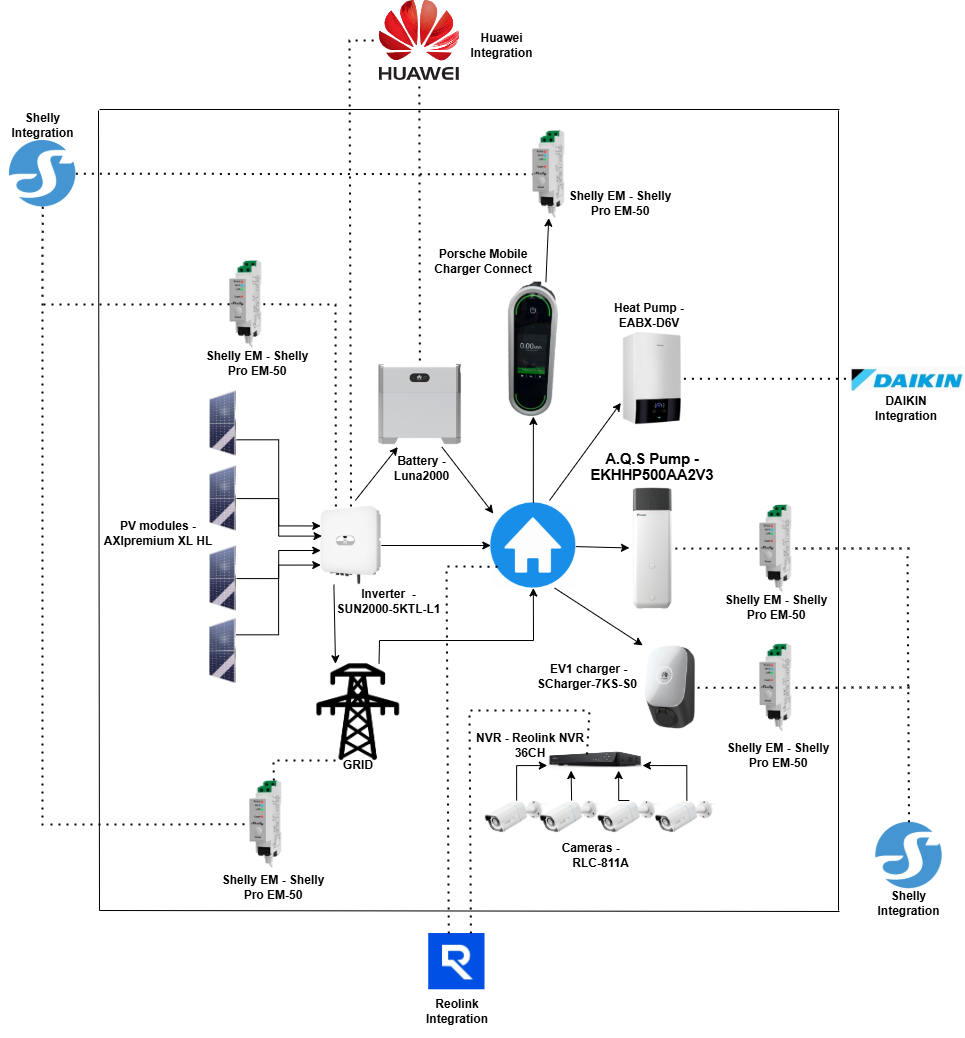
\includegraphics[width=\textwidth]{Smart_Home_Architecture.png}
	\caption{Smart Home - Architecture}
	\label{fig:Smart_Home_Architecture.png}
\end{figure}

Following we detail this architecture functioning:  
The diagram represents an integrated system for energy production, monitoring and management, air conditioning, electric vehicle charging and video surveillance, centralized in Home Assistant.

On the left of the diagram are the \textit{AXIpremium XL HL} photovoltaic modules, responsible for capturing solar energy. These panels are connected to the \textit{Huawei SUN2000-5KTL-L1} inverter, which converts the direct current (DC) generated by the panels into alternating current (AC) usable in the home's electrical grid. The inverter is also connected to the \textit{Huawei LUNA2000} battery, allowing excess solar energy to be stored for later consumption, such as at night or during periods of low solar production. Furthermore, the inverter connects directly to the electrical grid (GRID), enabling both the consumption of energy from the grid and the injection of excess energy. This entire energy production and storage system is monitored and integrated through \textit{Huawei Integration}, which allows energy flows to be monitored and managed.

\textit{Shelly EM} devices – \textit{Shelly Pro EM-50}, responsible for monitoring specific electrical consumption, were installed at various points in the system. One of these devices measures the overall consumption of the house, while the others monitor specific equipment: the \textit{Porsche Mobile Charger Connect} charger, the \textit{Daikin EABX-D6V} heat pump, the \textit{Daikin EKHHP500AA2V3} domestic hot water heat pump, the \textit{EV1 SCharger-7KS-S0} charger and the \textit{Reolink} video surveillance system (\textit{NVR} and cameras). These meters send consumption data to the home automation platform through \textit{Shelly Integration}, allowing for a detailed, real-time view of energy consumption and enabling smart automation.

On the right side of the diagram, \textit{Daikin} brand air conditioning equipment is represented. The \textit{EABX-D6V} heat pump, used for heating, and the \textit{EKHHP500AA2V3} heat pump, dedicated to the production of domestic hot water. Both equipment are integrated into the system through \textit{Daikin Integration}, which makes it possible to monitor their consumption and manage their operation in an optimized way.

The system also includes two electric vehicle chargers: the \textit{Porsche Mobile Charger Connect} (16A) and the \textit{SCharger-7KS-S0} (32A). These chargers are connected to the home's electrical grid and are monitored by \textit{Shelly} devices, allowing you to control their energy consumption and apply automations, such as prioritizing charging with excess solar energy or scheduling charging at times of lower energy costs.

The video surveillance component is provided by the \textit{Reolink} system, consisting of a \textit{Reolink 36CH NVR} and four \textit{Reolink RLC-811A} cameras. This system is connected to the local network and integrated through \textit{Reolink Integration}, allowing continuous monitoring and recording of security images.

In the center of the diagram is the house icon, which represents \textit{Home Assistant}.  
It acts as the brain of the system, integrating all platforms — \textit{Huawei}, \textit{Shelly}, \textit{Daikin} and \textit{Reolink} — and enabling real-time monitoring of energy production and consumption. Through this central system, it is possible to automatically control devices, such as air conditioning or chargers, and manage energy priorities, for example, ensuring that the electric car is only charged with surplus solar energy or switching off non-essential loads at times of highest consumption.

Overall, the diagram presents a complete, efficient and integrated solution for energy management, air conditioning, electric mobility and home security, with all components communicating with each other to maximize self-consumption, reduce waste and provide comfort and security.

\subsection{Equipments}

At the following subsections are described the equipments’ function and details.\\

The \textit{Daikin EKHHP500AA2V3} is a heat pump that produces domestic hot water, where the energy of the outside air is used to heat it. This makes it more efficient and sustainable than traditional electric or gas systems. The \textit{Daikin EABX-D6V}, on the other hand, is an indoor heat pump unit that is used for heating, domestic hot water (DHW), and cooling systems. This unit transfers thermal energy to the heating or DHW system through the thermal energy of the external unit and allows the production of domestic hot water.

For surveillance, the \textit{Reolink NVR 36CH} is a network video recorder that supports up to 36 IP cameras simultaneously, and also allows monitoring and management of the cameras, making it ideal for large surveillance installations. The \textit{Reolink RLC-811A} is an IP security camera suitable for outdoor use but can also be deployed indoors. It is powered by PoE, offering a reliable and efficient installation.

In the field of solar energy, the \textit{Huawei SUN2000-5KTL-L1} is a residential solar inverter with a rated power of 5\,kW, suitable for residential or small-scale installations. It offers high efficiency, supports battery integration, and includes smart monitoring. The \textit{Huawei LUNA2000} is a modular lithium-ion battery that stores excess solar energy, enabling the use of stored energy at night or when solar production is low, thus increasing self-consumption and reducing dependence on the power grid. Complementing this setup, the \textit{AXITEC AXIpremium XL HL} photovoltaic panels feature high-efficiency monocrystalline cells with half-cell technology. These panels perform better under partial shading, offer greater durability, and are suitable for installations that prioritize performance and efficiency.

For electric mobility, the \textit{SolaX Power SCharger-7KS-S0} is a 7.2\,kW electric vehicle charger that provides fast and safe charging. It integrates seamlessly with photovoltaic systems, prioritizing solar energy for charging. The \textit{Porsche Mobile Charger Connect} is a smart, portable charger for electric vehicles that allows charging at home or on the go via domestic or industrial sockets. It can be used as a mobile solution or permanently installed, and includes network connectivity for remote management and smart home integration.

For automation and control, devices from the \textit{Shelly} ecosystem were used. The \textit{Shelly 1PM Gen4} was installed to control the garage door, enabling wireless opening and closing through the Home Assistant interface. Additionally, several \textit{Shelly 2.5} modules were installed for the control of electric blinds, allowing both manual and automated movement control integrated in the dashboard.

For indoor climate control, five \textit{TADO Wired Smart Thermostats} were deployed. These devices allow real-time monitoring and regulation of temperature and humidity across multiple rooms, offering configurable heating and cooling modes and full integration with the central automation system.

Finally, the environmental sensing system was based on four devices from \textit{Netatmo}: the \textit{Netatmo Weather Station}, the \textit{Netatmo Smart Indoor Camera}, the \textit{Netatmo Wind Gauge}, and the \textit{Netatmo Rain Gauge}. This setup enables the continuous monitoring of atmospheric pressure, noise levels, and carbon dioxide concentration, enhancing user comfort and air quality management through data visualisation in the dashboard.


\subsection{Home Assistant and Hardware Requirements}

To run Home Assistant (HA), the following are the minimum hardware requirements depending on the installation method:

\begin{itemize}
    \item \textbf{Virtual Machine (VM):}
    \begin{itemize}
        \item At least 2\,CPU cores;
        \item 2\,GB RAM (4\,GB recommended for better performance);
        \item 32\,GB of disk space;
        \item Network adapter with internet access.
    \end{itemize}
    Installation guide for VM can be found at:\\
    \texttt{https://www.home-assistant.io/installation/windows}
    \\
    \item \textbf{Raspberry Pi (Recommended: Raspberry Pi 4):}
    \begin{itemize}
        \item Raspberry Pi 4 (2\,GB minimum, 4\,GB or 8\,GB recommended);
        \item microSD card (32\,GB minimum, or SSD via USB for better reliability);
        \item Power supply (official 3A USB-C recommended);
        \item Ethernet or Wi-Fi connection.
    \end{itemize}
    Installation guide for Raspberry Pi can be found at:\\
    \texttt{https://www.home-assistant.io/installation/raspberrypi}
\end{itemize}

For the initial installation of Home Assistant, we opted to use a virtual machine with 32GB disk space, 4GB RAM, 2 CPU and for the newtwork adapter we used NAT.

Later in the project, our instructor provided us with access to his public Home Assistant instance, allowing us to collaborate in real time on the same environment. This setup made teamwork and shared development significantly easier.

\subsection{Implementation}
With the communication scheme of the devices defined, Fig.~1, and all devices connected to the Wi-Fi network, the customization of our dashboard using cards began.\\

Some devices, such as the \textit{Shelly}, were automatically detected by the native integration of \textit{Home Assistant}, which demonstrates how the tool is already quite developed.

It started with the integration of the cameras. First, it was necessary to associate the cameras with the \textit{Reolink} integration, already available on the \textit{Home Assistant} platform, where it was enough to enter the username, password, and IP address of the device.

The same principle was used for the \textit{Daikin Onecta} devices, heat pump and DHW pump, where to complete the integration it was necessary to provide the account name, client ID, and client secret.

Finally, before customizing our dashboard, we installed what is perhaps the most important tool of \textit{Home Assistant}, \textit{HACS} (Home Assistant Community Store).

It is in this store that we installed the \textit{Huawei Solar} integration, necessary to integrate the \textit{Huawei SUN2000-5KTL}. To complete the configuration, the connection was set to network, entering the inverter’s IP address and communication port, allowing access to its sensors via the \textit{Modbus TCP} protocol. Both the inverter and the \textit{LUNA2000} battery were integrated through this same \textit{Huawei} integration.

Also in \textit{HACS}, we installed the power-flow-card-plus, the card that allows us to clearly visualize the energy flows between the various devices.

After these configurations, we began customizing our dashboard. For the cameras, we used the image card in live mode, where we added 3 cameras. For energy monitoring, the sensors previously configured in the integrations were used, such as those from \textit{Shelly}, \textit{Daikin}, and \textit{Huawei}. Finally, for more convenient access to heating, the thermostat card and entities card were used to display some additional information.\\


%\section{Results}\label{sec:results}
%
%At this section we can see the results achieved with the implementation of these dashboards. 
%
%
%
%
%
%
%With the development of this project, it will also be possible to add a quantity of statistical information, which allows a necessary comparison between the results for different courses.

\section{Results}\label{sec:Results}
The following section detail the final result for each dashboard. 
\subsection{Main dashboard}

\begin{figure}[H] 
	\centering
	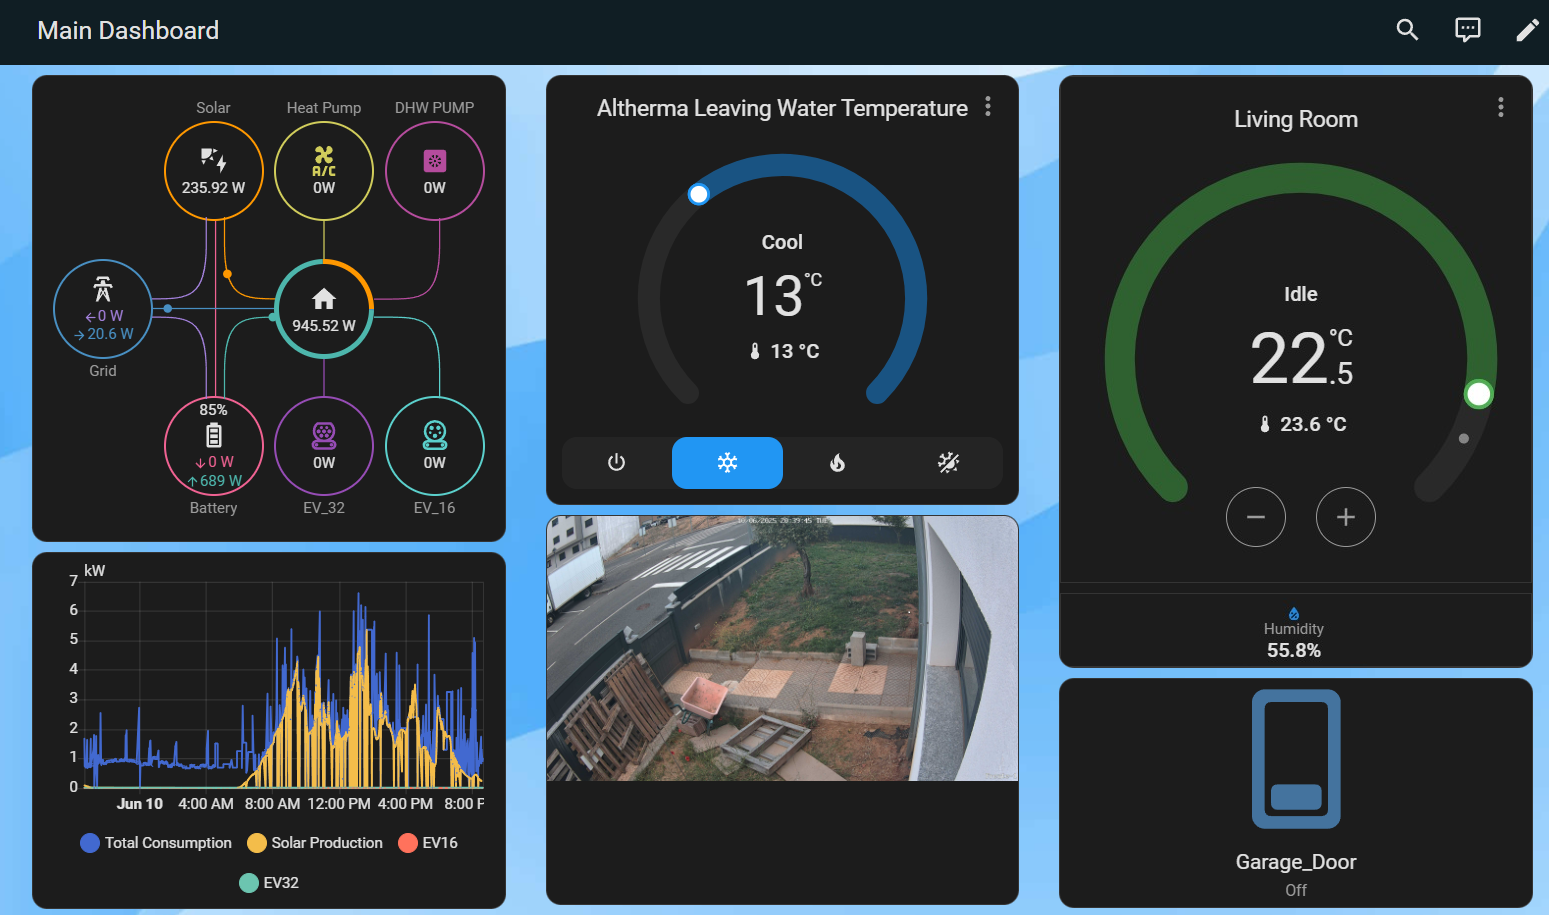
\includegraphics[width=\textwidth]{main.png}
	\caption{Main dashboard}
	\label{fig:main.png}
\end{figure}

As can be seen in Fig.~\ref{fig:main.png}, the dashboard was designed to be simple and practical, ensuring easy reading of the data. It is divided into three sections: the right area is dedicated to the living room thermostat and a button for the garage door. The left part is entirely dedicated to energy, where, at the top, the energy flow can be observed and, at the bottom, a graph presents the total consumption, solar production, and the consumption of the two vehicle chargers, of 16 and 32 amperes, over the last 24 hours. The central section is related to the heat pump, allowing the user to view its respective temperature and directly adjust the water outlet temperature. In addition, it includes a real-time view of the front door camera, offering direct control and monitoring of the main entrance of the house for greater security and convenience.

With the dashboard implemented, it is possible to ensure effective control of the front exterior area of the house through continuous monitoring of the security cameras. This guarantees a higher level of security when compared to a house without this IoT system. Additionally, it is possible to monitor the temperature and humidity of the living room, currently at 22.5ºC and 55.8 \%, respectively, and adjust the desired temperature. In the upper central part of the dashboard, we can verify that the heat pump is currently in cooling mode at 13ºC.

On the left part of the dashboard, we can observe that, at this moment, the house is consuming a total of 945.92 W, of which 253.92 W comes from solar production, 20.6 W comes from the electrical grid, and the battery is supplying 689 W to the house. This quick and intuitive access to energy information allows the user to better manage energy consumption, being able, for example, to choose to postpone the charging of the electric vehicle until an increase in solar production is observed.

This is just one of the countless possibilities for customizing dashboards in Home Assistant, which can be adapted to the specific needs of each user.


\subsection{Energy dashboard}

\begin{figure}[H] 
	\centering
	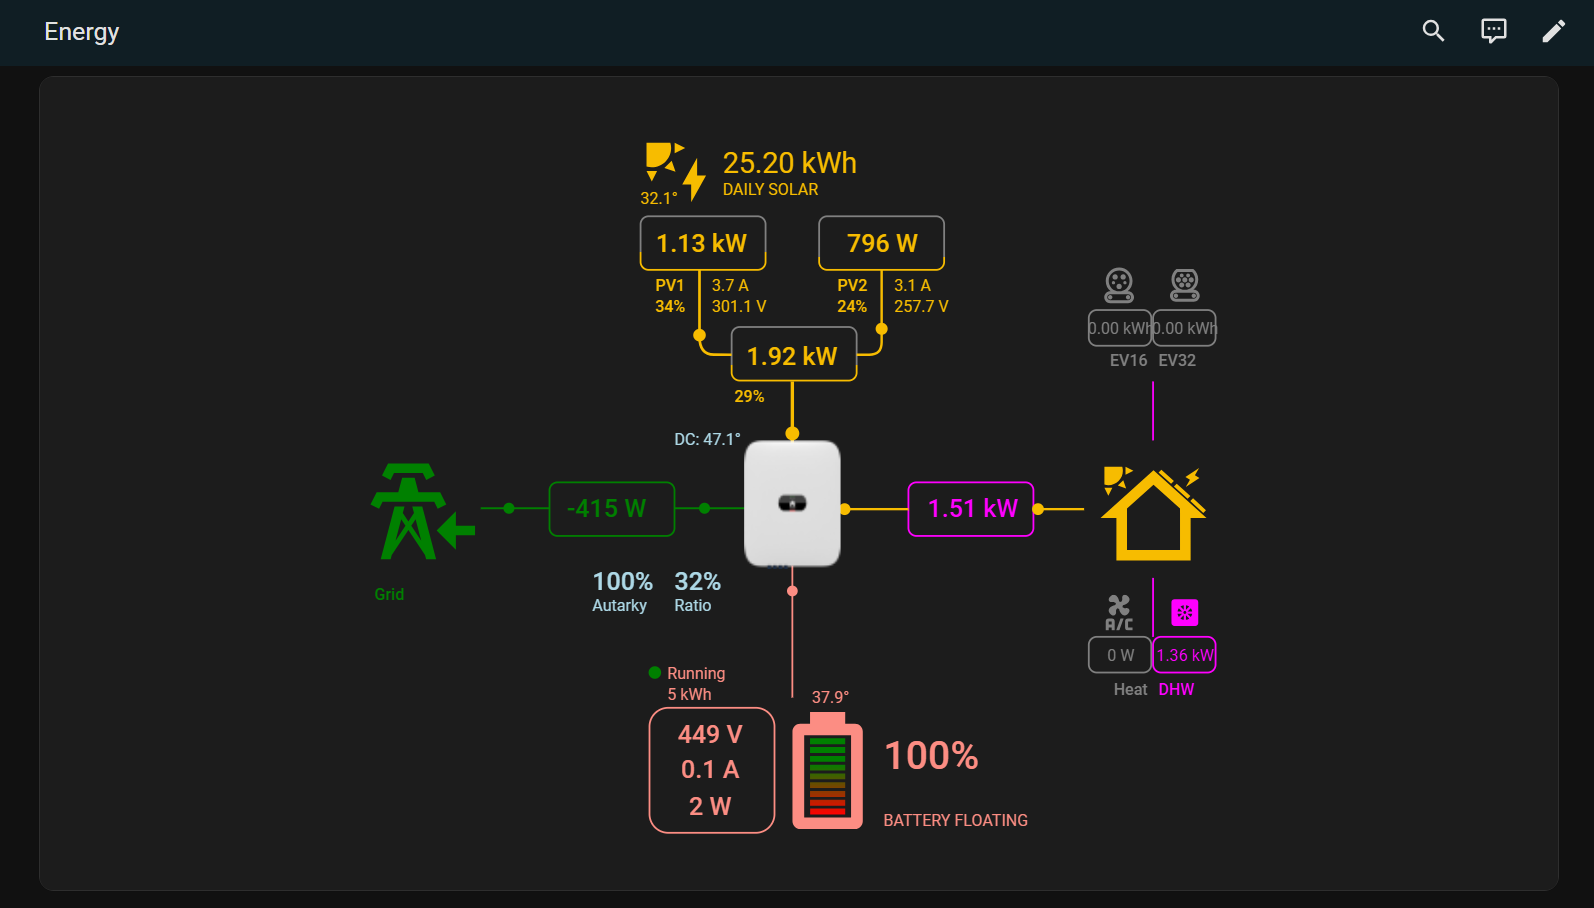
\includegraphics[width=\textwidth]{energy.png}
	\caption{Energy dashboard}
	\label{fig:energy.png}
\end{figure}

Fig.~\ref{fig:energy.png} presents the dashboard dedicated to energy monitoring, developed using the \textit{Sunsynk Power Flow Card}, a visual and animated card suitable for the \textit{Huawei} inverter. In this way, the understanding of the real-time energy flow becomes simpler and clearer.
At the center of the image is the \textit{Huawei} inverter, responsible for the system's energy management. Connected to it are the solar panels, the electrical grid (grid), the battery storage system, and the household load.
The system has two independent photovoltaic systems, designated PV1 (1.13 kW) and PV2 (796 W), totaling 1.92 kW of instantaneous production. This configuration allows for the monitoring of individual production from each system (PV1 or PV2), as well as the total production.
The grid can assume two states: energy import, represented by positive values, or energy export, represented by negative values, such as the -415 W shown in the image, indicating energy surplus.
Just like the grid, the battery is bidirectional, showing positive values when charging and negative values when discharging. In the situation presented, the battery is at 100\% capacity and in floating mode.
Finally, the total household consumption is 1.51 kW, a value derived from the sum of all energy sources available at the moment (solar panels, electrical grid, and battery). We can also see the main energy-consuming devices in the house, with emphasis on the two electric chargers (EV16 and EV32). The remaining two devices are the heat pump and the DHW pump, the latter of which is currently drawing 136 kW.

\subsection{Cameras dashboard}

\begin{figure}[H] 
	\centering
	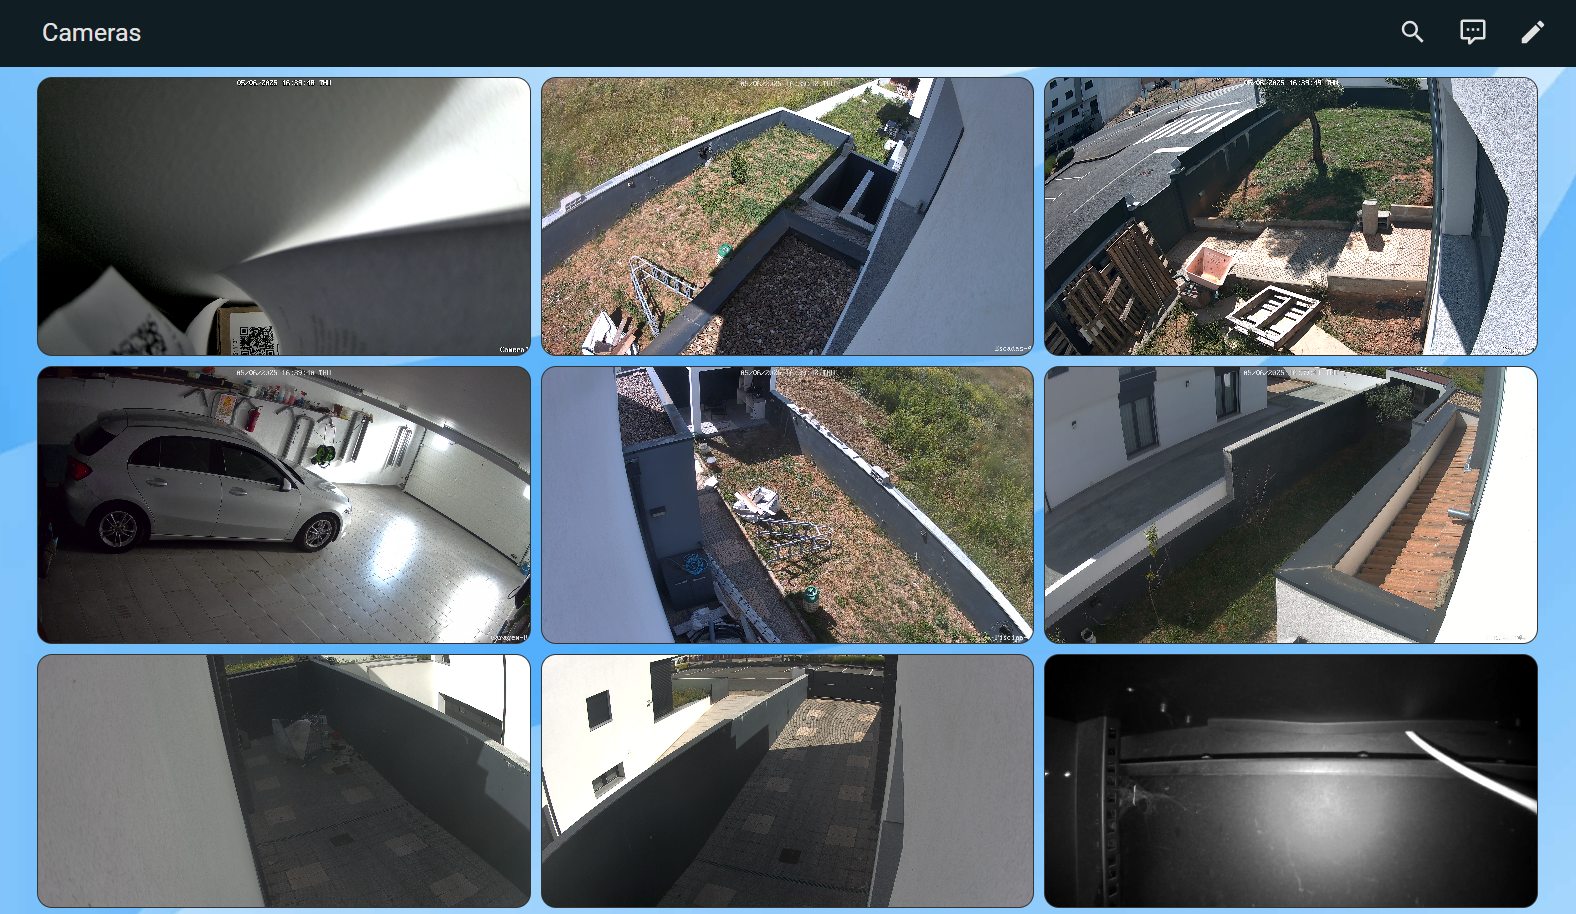
\includegraphics[width=\textwidth]{nvr.png}
	\caption{Cameras dashboard}
	\label{fig:nvr.png}
\end{figure}

As shown in Fig.~\ref{fig:nvr.png}, this dashboard is entirely dedicated to the real-time monitoring of the property's surveillance system. It presents a structured grid layout with nine camera feeds, covering various outdoor areas. The cameras capture different perspectives of the surroundings, including access paths, side walls, and perimeter zones. The center image on the second row clearly displays the garage interior. Notably, the bottom-right camera feed corresponds to a Netatmo integration, which provides additional coverage with smart detection capabilities. This setup provides full visual coverage of the exterior environment, enhancing security and allowing the user to quickly assess any activity around the property. The layout is clean and efficient, offering immediate access to all camera views for effective home surveillance.

\subsection{TADO dashboard}

\begin{figure}[H] 
	\centering
	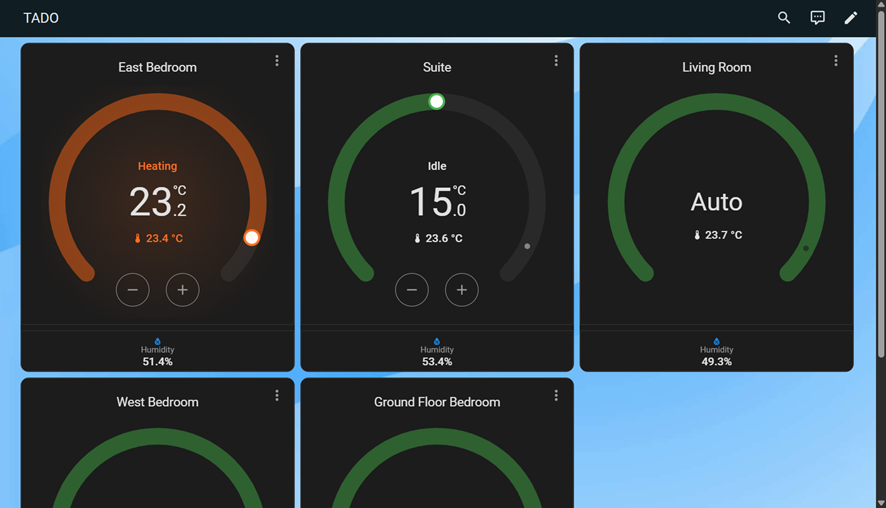
\includegraphics[width=\textwidth]{Tado.png}
	\caption{Tado Dashboard}
	\label{fig:Tado.png}
\end{figure}

Fig.~\ref{fig:Tado.png} provides a comprehensive overview of the indoor climate control system, displaying the current status of thermostats across various rooms in the house. Each card shows the current temperature, relative humidity, and the configured operating mode (e.g., \textit{Auto} or manual setpoint).
Here's a breakdown of the displayed data:

\begin{itemize}
    \item \textbf{East Bedroom}: The current temperature is 23.4\,°C, and the thermostat is set to a manual target of 23.2\,°C. The humidity is 51.4\%.
    
    \item \textbf{Suite}: The thermostat is set to a much lower target temperature of 15.0\,°C, while the room’s actual temperature is 23.6\,°C, with 51.8\% humidity.
    
    \item \textbf{Living Room}: Target temperature is Auto, with an actual temperature of 23.7\,°C and 49.3\% humidity.
\end{itemize}

To check the West Bedroom and the Ground Floor Bedroom, it is possible to scroll down the page.

This interface provides both real-time visibility and control over the thermal conditions in each area of the home. It supports energy efficiency by enabling the user to adapt the climate system only where needed, and to identify rooms with inconsistent temperature or humidity levels.

\subsection{Pumps Dashboard}

\begin{figure}[H] 
	\centering
	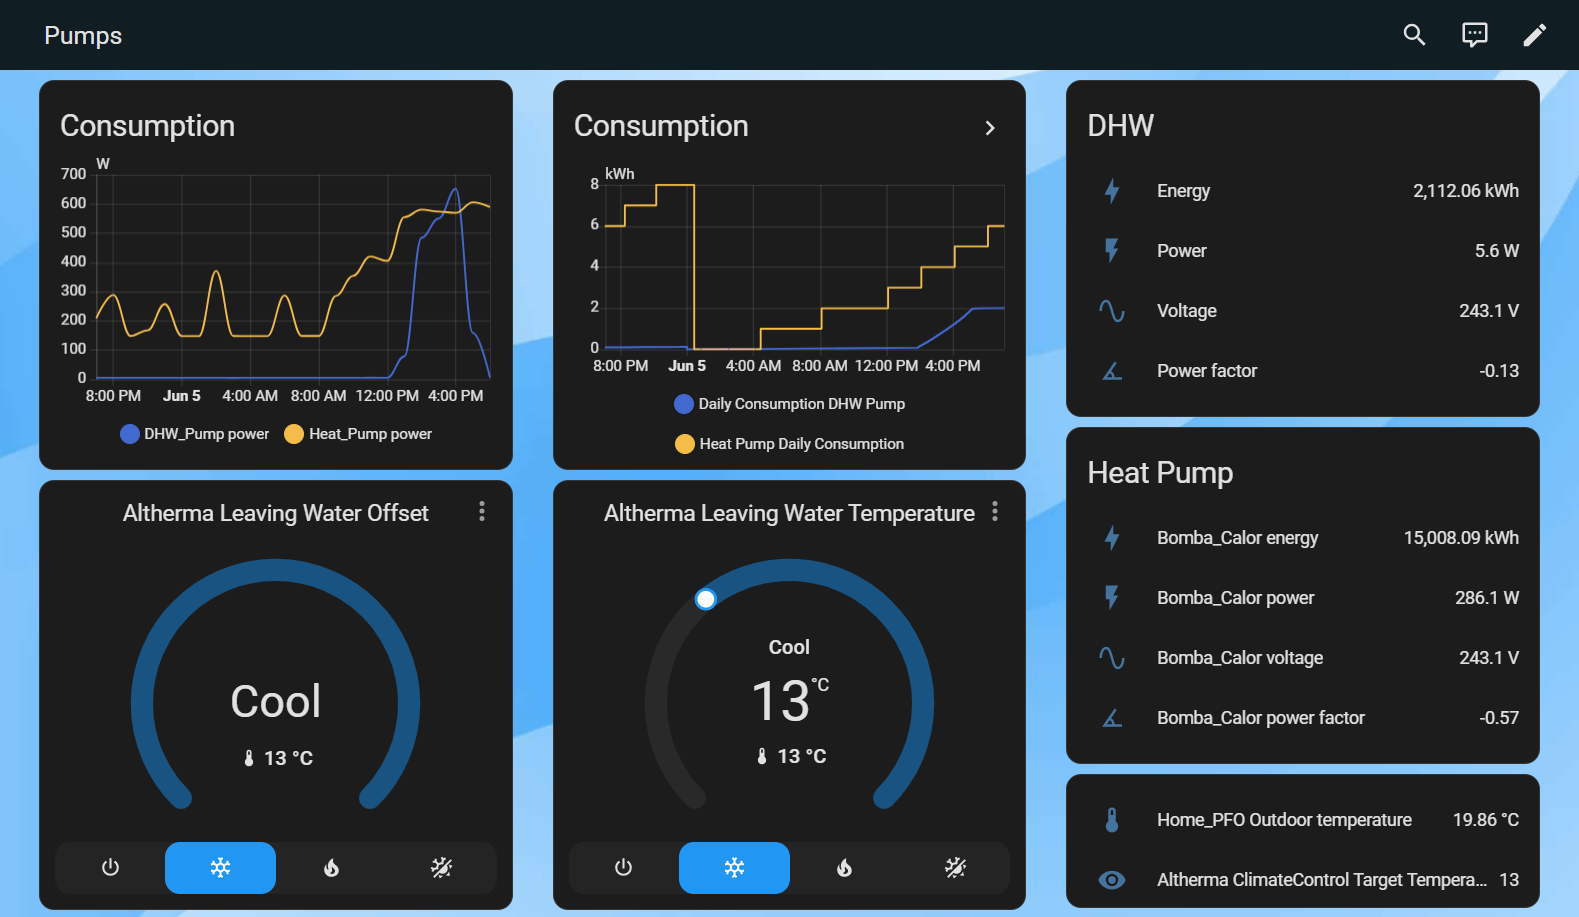
\includegraphics[width=\textwidth]{bombas.png}
	\caption{Main dashboard of the heating and domestic hot water pumps}
	\label{fig:bombas}
\end{figure}

The interface shown in Fig.~\ref{fig:bombas} provides a clear and organized overview of the heating system, focusing on the \textit{Altherma} heat pump and the domestic hot water pump (DHW). The dashboard is divided into several key components:

\begin{itemize}
    \item \textbf{Daily Consumption and Power Charts}:
    \begin{itemize}
        \item \textbf{Heat Pump Daily Consumption}: a complementary graph that reinforces the analysis of the Altherma system’s daily energy usage.
        \item \textbf{DHW Pump Daily Consumption}: displays the daily consumption of the DHW pump, with a steady increase throughout the day, surpassing 8 kWh.
        \item \textbf{DHW Pump power}: shows the power consumption of the DHW pump, reaching values above 500 W.
        \item \textbf{Heat Pump power}: shows the power consumption of the heat pump, currently around 1132.9 W.
    \end{itemize}

    \item \textbf{Temperature and Mode Controls} (bottom left): Two control cards allow direct adjustment of the pump temperature and operating mode:
    \begin{itemize}
        \item \textbf{Heating}: set to 35 ºC, currently in \textit{Cooling} mode, with water outlet temperature set to 13 ºC.
        \item \textbf{Cooling}: also set to 13 ºC, with the system actively operating in cooling mode.
    \end{itemize}

    \item \textbf{Additional information} (right): Displays complementary system metrics such as DHW energy consumption (2110.11 kWh), power (7.1 W), voltage (241.6 V), and power factor (-0.17). For the heat pump, the energy usage is 15003.56 kWh, with a current power draw of 1132.9 W, voltage of 241.6 V, and power factor of -0.91. The outdoor temperature is 14.41~\textdegree{}C, and the Altherma target temperature is currently set to 13~\textdegree{}C.


\end{itemize}

\subsection{Blinds Dashboard}

\begin{figure}[H] 
	\centering
	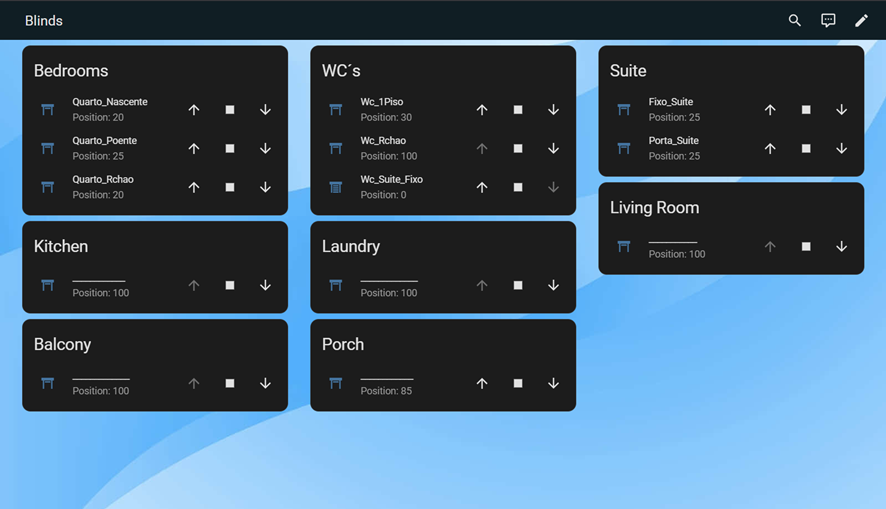
\includegraphics[width=\textwidth]{blinds.png}
	\caption{Blinds Dashboard}
	\label{fig:blinds}
\end{figure}

Fig.~\ref{fig:blinds} shows the complete dashboard interface for controlling the window blinds throughout the house. Each card corresponds to a specific room or area (e.g., \textit{Bedrooms}, \textit{Kitchen}, \textit{WC's}), and displays the individual blinds associated with that location.

For each blind, the current opening level is displayed (\texttt{Position: x}), where "0" represents fully closed and "100" fully open. The interface provides manual control through three buttons:

\begin{itemize}
    \item \textbf{Up arrow}: opens the blind.
    \item \textbf{Square button}: stops the blind at its current position.
    \item \textbf{Down arrow}: closes the blind.
\end{itemize}

Rooms with multiple blinds (such as the \textit{Suite} or \textit{Bed Rooms}) display each device individually with its corresponding name. The layout is responsive and designed for quick visual identification and manual control of all automated blinds in the home.

\subsection{Netatmo Dashboard}

\begin{figure}[H] 
	\centering
	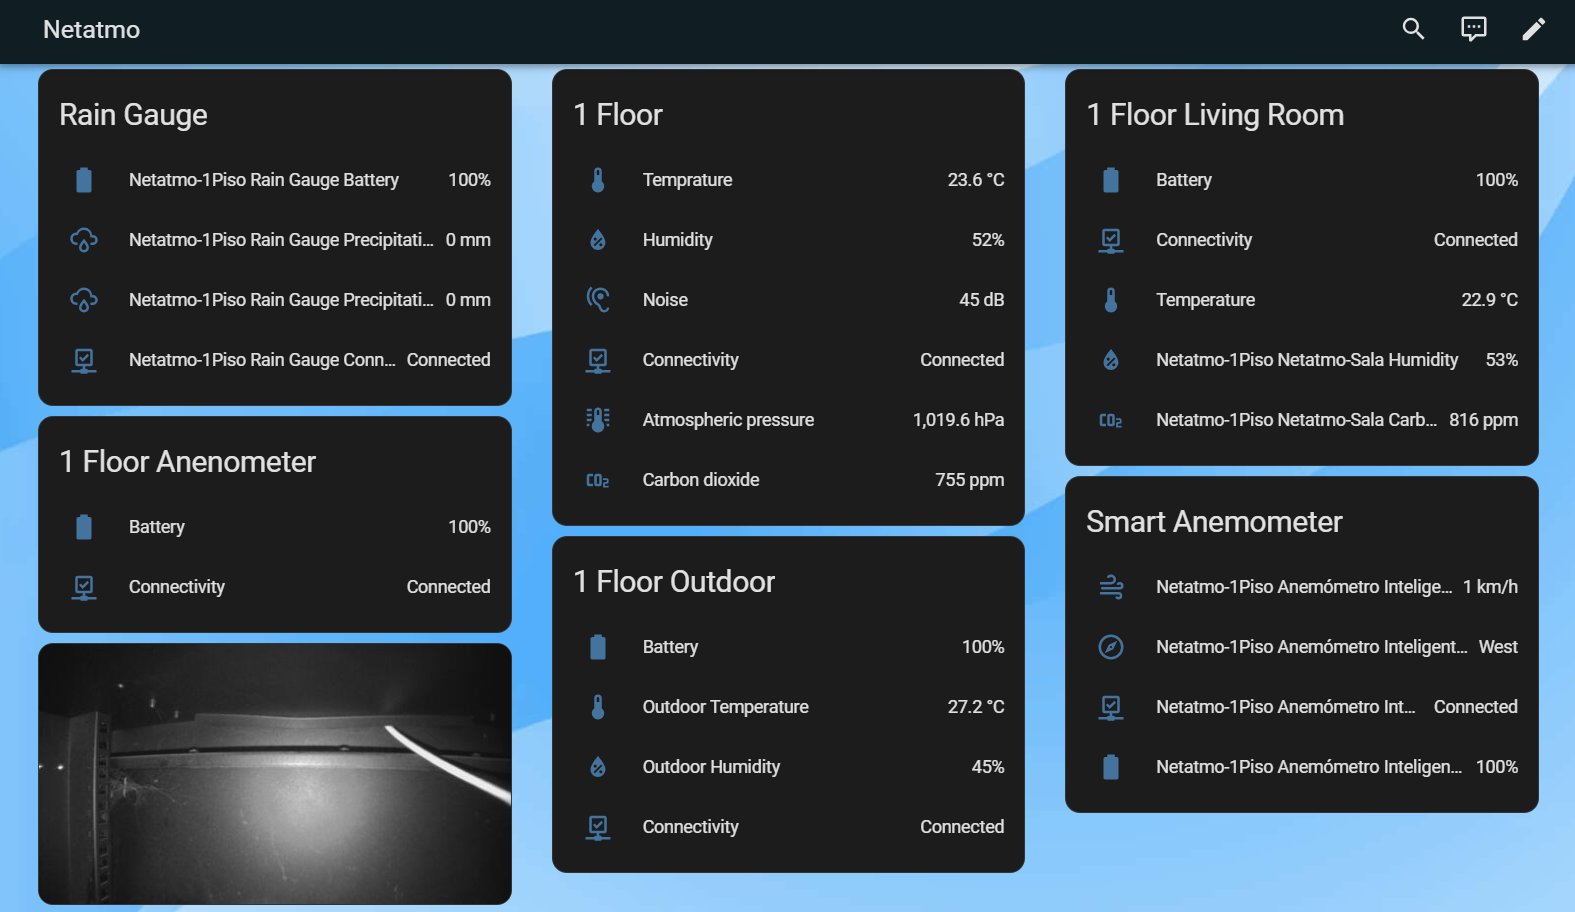
\includegraphics[width=\textwidth]{netatmo.png}
	\caption{Netatmo Dashboard}
	\label{fig:netatmo}
\end{figure}

Fig.~\ref{fig:netatmo}, which provides a compact overview of several environmental sensors placed throughout the home. At the top left, a camera feed monitors the sensor installation area. The central card displays the main indoor module located on the first floor, with readings such as temperature (23.6°C), humidity (52\%), noise (45 dB), atmospheric pressure (1019.6 hPa), and CO2 level (755 ppm), all with active connectivity.

The anemometer module on the first floor is fully connected and reports a 100\% battery level. In the living room, the indoor module is also connected, showing 100\% battery, temperature of 22.9°C, humidity of 53\%, and a CO2 level of 816 ppm. The outdoor module indicates 27.2°C and 45\% humidity, also with 100\% battery and active connectivity. Additionally, the smart anemometer reports a wind speed of 1 km/h, direction West, full battery, and active connection.

This dashboard allows quick and centralized access to indoor air quality and weather data, enhancing control and monitoring in smart home environments.

 

\section{Conclusions}\label{sec:Conclusion}

In summary, our project was able to leverage Home Assistant by implementing automation tools and open platforms to simplify the management and monitoring of residential environments. We managed to resolve common challenges related to device compatibility, decentralization, and lack of unified control, creating an integrated and easy-to-use solution for users.

With this project, the goal was achieved, a single, easy-to-understand dashboard that connects several smart devices, including photovoltaic systems, energy storage solutions, electric vehicle chargers, heating and cooling systems, and video surveillance. Since the communication of these devices is exclusively via Wi-Fi, and within our private network, it was possible to ensure that our data always stayed on our network without relying on the cloud.

The impact of our project goes beyond mere convenience. Users now have the ability to make more informed decisions, better utilize solar energy, and even reduce dependence on the electrical grid. We also made the home safer and more comfortable by integrating surveillance cameras and climate control into the same interface. The simple dashboard facilitates the visualization and interaction with the system, allowing all types of users to access, monitor, and manage their automation system with clarity, quick information, and adaptable controls, even without technical knowledge.

Upon completing the project, we highlighted the results achieved and the potential of the solution. Future work may include the integration of additional devices and services, the evaluation of the use of artificial intelligence to anticipate and automate processes, and the collection of user feedback to further improve the dashboards and automations. Due to its flexibility, Home Assistant can continuously evolve, ensuring that the system keeps pace with technological advances and user needs. This project proves that the solution is effective and offers many features within an open-source approach that respects privacy, promoting a more sustainable, efficient, and secure living environment.



\nocite{*}
\bibliographystyle{spmpsci}

\bibliography{references_PFO}

%\input{references}
\end{document}